\section{Methods}

The purpose of this study is to demonstrate that using a model-based approach we can track EEG dynamics in real-time. If we assume that the model we are using is a good model of the system we are recording from, we can then also conclude that the results obtained have physiological meaning, and will allow further insight into the mechanisms involved in seizure generation and termination. We approach the problem of tracking enural dynamics by using two types of models: an \textsl{in-vivo} model of focal temporal lobe epilepsy with a hippocampal seizure focus, and a computational model of the hippocampus.

\subsection{\textsl{In-vivo} Model of Focal Epilepsy}

In this study, we make use of an \textsl{in-vivo} model of focal temporal lobe epilepsy. Epilepsy is induced in these animals by injecting tetanus toxin into the CA3 region of their hippocampus~\citep{jefferys1995chronic}. This particular model was chosen as it has a localised seizure focus, and results in the animals having seizure events that are similar to the electrophysiological and physical symptoms observed in human patients with temporal lobe epilepsy. 

Sprague Dawley rats~(300-400 grams) are injected with $0.4-0.6\mu l$ of tetanus toxin. The tetanus toxin is injected into the CA3 region of the left hippocampus - $-3.5mm$ anterior-posterior (AP), $3mm$ medial lateral and $-3.5mm$ dorsal ventral (DV) relative to bregma. Four electrodes are placed to record local field potentials: a twisted pair electrode is inserted into the same location as the tetanus toxin, and two screw electrodes are placed on the surface of the cortex on the right hemisphere. A cerebellar electrode is placed as a reference for all electrodes. Electrodes are connected to a pedestal and held in place by dental cement. The animals are left to recover for five to seven days, and are recorded from for 24 hours a day for six to eight weeks. All animal experiments are done under the approval of an ethics committee.

\subsection{Neural Mass Model} 

All neural field models can be described by a temporal and spatial response curve, and a function that relates membrane potentials to firing rates. For neural mass models the spatial element is removed from this general description such that

\begin{equation}\label{eq:conv_eq}
    v_n(t) = \frac{\alpha_{mn}}{\tau_{mn}}\int_{-\infty}^t  h_{mn}(t-t')g(v_m(t')) \,\mathrm{d}t' + v_r,
\end{equation}
where $\alpha_{mn}$ is a measure of the connectivity and synaptic strength between populations $m$ and $n$, $h_{mn}(t)$ is the temporal response curve - commonly referred to as a post synaptic response kernel - $\tau_{mn}$ is the time constant which indicates the average propagation delay between populations $m$ and $n$ and $v_r$ is the resting membrane potential. The temporal response curve (Figure~\ref{fig: Simple}) is a time delayed exponential decay function:
\begin{equation}
    h_{mn}(t) = \eta(t)t\exp\left(-\frac{t}{\tau_{mn}}\right),
\end{equation}
where $\eta(t)$ is the Heaviside step function. 

\begin{figure}
	\centering
		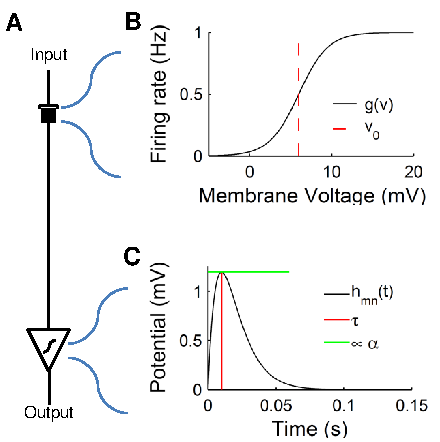
\includegraphics{Biological_Response.pdf}
	\caption{Simple Neural Mass Model. (\textbf{A}) An example of a simple neural mass model. This model consists of a single neural population - the triangle - and a single synapse - the square block. (\textbf{B}) Temporal response curve for a synapse. The black line demonstrates the response of a synapse to an impulse response. The time constant ($\tau$) and synaptic gain ($\alpha$) are demonstrated in this figure. The peak response of this function is $\alpha \exp(-1)$ and the time at which this peak occurs is equal to $\tau$. (\textbf{C}) Somatic response curve. The black line indicates the function $g(v)$ which is a sigmoidal activation curve. This function demonstrates the resulting normalized firing rate produced by a neural population as a function of the membrane potential over it. In this figure $v_{0}$ is the membrane potential at which the firing rate produced is half its maximum.}
	\label{fig: Simple}
\end{figure}

The firing rate of each population is determined from a sigmoid function~(Figure~\ref{fig: Simple}), that models the action of a population of soma's. The sigmoid function translates the membrane potential of a population to its aggregate firing rate,
\begin{align}\label{eq:sigmoid}
    g\left(v_n(t)\right) =& \frac{1}{1+\exp{\left(\varsigma_n\left(v_{0n} - v_n(t)\right)\right)}}.
\end{align}
The quantity $\varsigma_n$ describes the gradient of the sigmoid activation curve and $v_{0n}$ the membrane potential that results in half the maximum firing rate. The constant $v_{0n}$ is a lumped parameter, that includes the effect of the resting membrane potential on the activation curve. 

The convolution in Equation~\ref{eq:conv_eq} can also be written as an ordinary differential equation (ODE)
\begin{equation}\label{eq:2ndOrder}
    \mathrm{D}v_n(t) = \frac{\mathrm{d}^2 v_n(t)}{\mathrm{d}t^2} + \frac{2}{\tau_{mn}}\frac{\mathrm{d} v_n(t)}{\mathrm{d}t} + \frac{1}{\tau_{mn}^2} v_n(t) = \frac{\alpha_{mn}}{\tau_{mn}} g(v_m(t)),
\end{equation}
where $\mathrm{D}$ is a differential operator. Equation~\ref{eq:2ndOrder} can be written as two partial differential equations
\begin{equation} \label{eq:2ndOrderNMM}
    \frac{\mathrm{d} v_n(t)}{\mathrm{d}t} = z_n(t),\,\,\,\,\,    \frac{\mathrm{d}z_n(t)}{\mathrm{d}t} = \frac{\alpha_{mn}}{\tau_{mn}} g(v_m(t)) - \frac{2}{\tau_{mn}}z_n(t) - \frac{1}{\tau_{mn}^2} v_n(t),
\end{equation}
where $z_n(t)$ is the time derivative of $v_n(t)$. These two partial differential equations form the basis of a state-space model for all neural masses.

The simplest possible neural mass model has a single population with a single input and output firing rate~(Figure~\ref{fig: Simple}). This model consists of a single post synaptic response curve and a sigmoid function.

In this study, we consider the neural mass model of the hippocampus (Figure~\ref{fig: Biological}). This is an expansion of the simple model (Figure~\ref{fig: Simple}) where four populations - two excitatory and two inhibitory - are included. Each populations post synaptic response curve is described by a time constant ($\tau_{mn}$) and synaptic gain ($\alpha_{mn}$). Here we make the assumption that the time constants of all the populations are stationary (Table~\ref{tab: Static}) and that the synaptic gains are time varying. This assumption has been shown to still allow the model we are considering to mimic EEG recorded from the hippocampus. The assumption that the time constants are static and the synaptic gains are time varying is the same as assuming that the modeled synapse are current rather than conductance based. All populations in the model are connected by different number of synapses. The number of these synaptic connections is represented by a connectivity constant ($c_{1-7}$). The last element of the model is its input which represents the firing rate to the modeled population from the rest of the brain, and is modeled as a Gaussian noise source with a non-zero mean.

A further assumption made in this study is that all excitatory temporal response curves have the same description, that is:
\begin{equation}\label{eq:ExcSynapse}
    \alpha_{\mathrm{pe}} = \alpha_{\mathrm{ps}} = \alpha_{\mathrm{pf}} = \alpha_{\mathrm{ep}} = \alpha_{\mathrm{ip}},\,\,\,\,\, \tau_{\mathrm{pe}} = \tau_{\mathrm{ps}} = \tau_{\mathrm{pf}} = \tau_{\mathrm{ep}} = \tau_{\mathrm{ip}},
\end{equation} where p, e, s, and f represent the pyramidal, excitatory, slow inhibitory and fast inhibitory populations and i the input into the model. The same assumption is also made for the slow inhibitory temporal response curve
		\begin{equation}\label{eq:InhSynapse}
		\alpha_{\mathrm{sf}} = \alpha_{\mathrm{sp}},\,\,\,\,\, \tau_{\mathrm{sf}} = \tau_{\mathrm{sp}}.
\end{equation}  By making this assumption we can reduce the number of synapse required to model this neural mass (Figure~\ref{fig: Biological}), while retaining all the dynamics in the model required to mimic recorded EEG. To simplify notation all excitatory temporal response curves will be specified by $\alpha_{\mathrm{p}}$ and $\tau_{\mathrm{p}}$, slow inhibitory by $\alpha_{\mathrm{s}}$ and $\tau_{\mathrm{s}}$ and fast inhibitory by $\alpha_{\mathrm{f}}$ and $\tau_{\mathrm{f}}$. 

Studies have shown that by altering the synaptic gains of this model recorded hippocampal EEG can be mimicked~\citep{wendling2002epileptic}. Therefore, we consider the estimation of $\alpha_{\mathrm{p}}$, $\alpha_{\mathrm{s}}$ and $\alpha_{\mathrm{f}}$. We also consider the estimation of an extra model parameter, the mean input firing rate. By adding this parameter, we can evaluate whether there are changes in network phenomena involved in seizures. All other parameters are considered to be static (Table~\ref{tab: Static}).

\singlespacing 
\footnotesize
\begin{center}%%%%%%%%%%%%%%%%%%%%%%%%%%%%%%%%%%%%%%%%%%
	\begin{table}
			\caption{Static Model Parameters~\citep{wendling2002epileptic}. Here p, e, s and f represent populations of pyramidal neurons and excitatory and slow and fast inhibitory interneurons, respectively.}
		\begin{tabular}{||p{2.5cm}|p{9cm}|p{1.2cm}|p{1cm}||}\hline
			 \textsc{Parameter}  & \textsc{Physical description} & \textsc{Value} & \textsc{Units}  \\\hline\hline
			 $\tau_{\mathrm{p}}$ & Time constant for excitatory temporal response curve & 100 & $s^{-1}$\\\hline
			 $\tau_{\mathrm{s}}$ & Time constant for slow inhibitory temporal response curve & 35 & $s^{-1}$\\\hline
			 $\tau_{\mathrm{f}}$ & Time constant for fast inhibitory temporal response curve & 500 & $s^{-1}$\\\hline
			 $C$ & Connectivity constant & 135 & NA\\\hline
			 $c_{1}$ & Connectivity constant (p - e) & $C$ & NA \\\hline
			 $c_{2}$ & Connectivity constant (e - p) & $0.8C$ & NA\\\hline
			 $c_{3}$ & Connectivity constant (p - s) & $0.25C$ & NA \\\hline
			 $c_{4}$ & Connectivity constant (s - p)& $0.25C$ & NA\\\hline
			 $c_{5}$ & Connectivity constant (p - f) & $0.3C$ & NA\\\hline
			 $c_{6}$ & Connectivity constant (s - f) & $0.1C$ & NA\\\hline
			 $c_{7}$ & Connectivity constant (f - p) & $0.8C$ & NA\\\hline
			 $g_{max}$ & Maximum firing rate & 5 & Hz \\\hline
			 $v_{0}$ & Membrane potential resulting in 50\% of maximal firing rate & 6 & $mV^{-1}$\\\hline
			 $\varsigma$ & Gradient of sigmoid function & 0.56 & NA \\\hline
		\end{tabular}
		\label{tab: Static}
	\end{table}
\end{center}%%%%%%%%%%%%%%%%%%%%%%%%%%%%%%%%%%%%%%%%%%%%%%%%%%%%%%%%%%
\doublespacing
\normalsize

 \begin{figure}
 	\centering
 		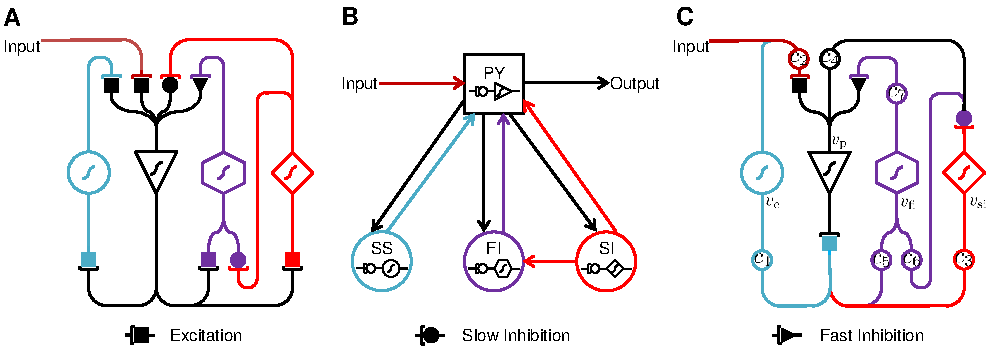
\includegraphics{fig/Biological_Model.pdf}
 	\caption{Graphical Description of the Neural Mass Model of the Hippocampus. (\textbf{A}) Graphical description of the neural mass model of the hippocampus. In this figure the traingle, circle diamond and hexagon represent populations of pyramidal, spiny stellate and slow and fast inhbitory neurons. Synaptic connections are specified by a u shaped structure, where the secondary terminal has different shapes depending on the response of the synapse. The 'input' specified in the figure is a firing rate from other cortical regions connected to the modelled area. (\textbf{B}) Flow diagram of the of the neural mass model of the hippocampus. (\textbf{C}) Simplified graphical description of the neural mass model of the hippocampus.}
 	\label{fig: Biological}
 \end{figure}


\subsection{Estimation}

\red{Generic description on a nonlinear system}

We begin by defining a generic non-linear system\begin{align}
\label{eqn: NonlinEstS}
\mathbf{\dot{x}}(t) &= \mathbf{A}(\mathbf{x}(t),\mathbf{\theta}(t)) + \mathbf{B}(\mathbf{u}(t)) + \mathbf{n}(t)\\
\label{eqn: NonlinEstO}
\mathbf{y}(t)  &= \mathbf{C}(\mathbf{x}(t)) +\mathbf{D}(\mathbf{u}(t))+\mathbf{r}(t),
\end{align} where boldface is used to indicate a matrix or vector. For a non-linear system boldface notation can also indicate a matrix of functions. Here, $\mathbf{x}(t)$ is the model states and $\dot{\mathbf{x}}(t)$ its derivative, where
\[ \mathbf{\dot{x}}(t) = \left[ \begin{array}[pos]{c}
\dot{x}_{1}(t)\\
\vdots \\
\dot{x}_{n}(t) \end{array} \right] .\] The state and input matrices are $\mathbf{A}$ and $\mathbf{B}$, respectively and $\mathbf{u}(t)$ is the model input. The observation and input-to-output matrices are $\mathbf{C}$ and $\mathbf{D}$, respectively. The model output is $\mathbf{y}(t)$ with $\mathbf{n}(t)$ the model uncertainty, and $\mathbf{r}(t)$ the observation noise. Here, $\mathbf{n}(t)$ is a bound on the expected model error, and $\mathbf{r}(t)$ describes the noise in the observations. Both $\mathbf{n}(t)$ and $\mathbf{r}(t)$ are zero mean Gaussian distributed with a system dependant variance. 


\red{Introduction to the UKF}

Estimation techniques attempt to approximate the model states given some observation. There are numerous techniques to achieve this, most of which are for linear systems. We make use of a nonlinear estimation technique, the unscented Kalman filter. This method consists of two steps: prediction and correction. The prediction step makes use of an unscented transform (Figure~\ref{fig: UKF}) to approximate the mean and covariance of the states after they have been propagated through the model. The correction step then determines the most likely states that best describes both the observation and the model prediction. This step makes use of the expected error on both the observations and the states to determine a weighting for each (Figure~\ref{fig: UKF}).

The unscented transform makes the assumption that the distribution of states before and after they are propagated through the model are Gaussian (Figure~\ref{fig: UKF}). The first step in the unscented transform involves drawing sigma points - points one standard deviation away from the mean - from a Gaussian distribution, 
\begin{align}\label{eqn: SigmaP}
\mathbf{\mathcal{X}}_{0} &= \mathbf{\overline{x}}_{k} \quad iff \quad \kappa >0\\
\mathbf{\mathcal{X}}_{n,k} &= \mathbf{\overline{x}}_{k} \pm (\sqrt{\kappa+D_{x}\mathbf{P_{xx,k}}})_{n} \quad n=1,\hdots,D_x,
\end{align} where $\mathbf{\mathcal{X}}_{n}$ represents the sigma points, $k$ the current sample, $\mathbf{\overline{x}}_{k}$ is the expected value of the state, $\mathbf{P_{xx,k}}$ is the covariance of the state and $D_{x}$ is the number of states in the system. This results in $2D_{x}$ sigma points. If $\kappa$ is greater than zero than the mean is also propagated through the model resulting in $2D_{x}+1$ sigma points. In general, the value of $\kappa$ is used to either scale up or scale down the effect of the mean on the unscented transform prediction. The notation $\sqrt{\cdot}_{n}$ is used to indicate the $n$th row of the matrix square root. 

The next step of the unscented transform involves propagating the sigma points through the model, and using the results to evaluate the statistics of the prediction,
\begin{align}\label{eqn: SigmaProp}%%%%%%%%%%%%%%%%%%%%%%%%%%%%%%%%%%%%
\mathbf{\mathcal{X}}_{n,k+1} &= \mathbf{\mathcal{X}}_{n,k}+ T(\mathbf{A}(\mathbf{\mathcal{X}}_{n,k}) +\mathbf{B}(\mathbf{u}_{k})) +\sqrt{T}{n}_{k}\\
\label{eqn: PriorSMean}
\overline{\mathbf{x}}_{k+1}^{-} &= \frac{1}{2D_{x}+\kappa}\sum_{n=0}^{2D_{x}} \mathbf{\mathcal{X}}_{n,k+1}\\
\label{eqn: PriorSCov}
\mathbf{P}_{xx,k+1}^{-} &= \frac{1}{2D_{x}+\kappa}\sum_{n=0}^{2D_{x}} (\mathbf{\mathcal{X}}_{n,k+1} -\mathbf{\overline{x}}_{k+1}^{-})(\mathbf{\mathcal{X}}_{n,k+1}-\mathbf{\overline{x}}_{k+1}^{-})^{\top} + \mathbf{Q},%%%%%%%%%%%%%%%%%%%%%%%%%%%%%%%%%%%%
\end{align} $\mathbf{\mathcal{X}}_{n,k+1}$ are the propagated sigma points, $\overline{\mathbf{x}}_{k+1}^{-}$ and $\mathbf{P}_{xx,k+1}^{-}$ are the predictions for the state and state covariance matrices. The negative superscript is used to indicate an uncorrected prediction. The term $\mathbf{Q}$ is the expectation of the model error $n_{k}$ and $(\cdot)^{\top}$ a matrix transpose. In this step, we have made use of a first order Euler-Maruyama approximation to propagate the model states one sample forward. This involves scaling the data by the sampling period ($T$), and the variance in the model by its square root.

From equations~\ref{eqn: SigmaProp}-\ref{eqn: PriorSCov} an expectation on the observed value can be determined. For a neural mass model the observation function is linear, so there is no need to propagate the prior distribution of model states through the observation function to determine the statistics of the prior estimate of the observation. Instead the statistics of the observation can be determined from the propagated sigma points,
\begin{align}
\mathbf{\mathcal{Y}}_{n,k+1} &= \mathbf{C}(\mathbf{\mathcal{X}}_{n,k+1})+ \mathbf{D}(\mathbf{u}_{k})+ \sqrt{T}\mathbf{r}_{k}\\
\overline{\mathbf{y}}_{k+1}^{-} &= \frac{1}{2D_{x}+\kappa}\sum_{n=1}^{2D_{x}} \mathbf{\mathcal{Y}}_{n,k+1}\\
\label{eqn: statecovg}
\mathbf{P}_{xy,k+1}^{-} &= \frac{1}{2D_{x}+\kappa}\sum_{n=1}^{2D_{x}} (\mathbf{\mathcal{X}}_{n,k+1}-\overline{\mathbf{x}}_{n,k+1}) (\mathbf{\mathcal{Y}}_{n,k+1}-\overline{\mathbf{y}}_{k+1}^{-})^{\top}\\
\mathbf{P}_{yy,k+1}^{-} &= \frac{1}{2D_{x}+\kappa}\sum_{n=1}^{2D_{x}} (\mathbf{\mathcal{Y}}_{n,k+1}-\overline{\mathbf{y}}_{k+1}^{-}) (\mathbf{\mathcal{Y}}_{n,k+1}-\overline{\mathbf{y}}_{k+1}^{-})^{\top} +\mathbf{R},%%%%%%%%%%%%%%%%%%%%%%%%%%%%%%%%%%%%%%%%%%%%
\end{align} where $\mathbf{\mathcal{Y}}_{n,k+1}$ are the predicted observations from all the sigma points, and $\overline{\mathbf{y}}_{k+1}^{-}$ and $\mathbf{P}_{yy,k+1}^{-}$ are the predictions for the model output and its covariance, respectively. The covariance matrix of the states and observations are $\mathbf{P}_{xy,k+1}^{-}$ and $\mathbf{R}$ is the expectation of the observation error $\mathbf{r}_{k}$.

In the correction step we make use of the knowledge of our prior distribution on states and the observations, as well as there expected value, and compare this to the experimental observation to improve our prediction. This is achieved using the standard formulation of the Kalman filter correction step,
\begin{align}
\mathbf{K} &= \mathbf{P}_{xy,k+1}^{-}(\mathbf{P}_{yy,k+1}^{-})^{-1}\\
\overline{\mathbf{x}}_{k+1} &= \overline{\mathbf{x}}_{k+1}^{-} + \mathbf{K}(\mathbf{y}_{k+1}-\overline{\mathbf{y}}_{k+1}^{-})\\
\mathbf{P}_{xx,k+1} &= \mathbf{P}_{xx,k+1}^{-} - \mathbf{K}(\mathbf{P}_{xy,k+1}^{-})^{\top},
\end{align} where $\mathbf{y}_{k}$ is the observation, $\overline{\mathbf{x}}_{k+1}$ is the corrected estimate of the state and $\mathbf{P}_{xx,k+1}$ is the estimate of its error.

 \begin{figure}
 	\centering
 		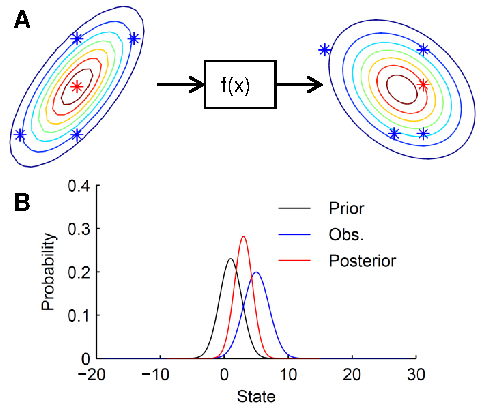
\includegraphics{fig/UnscentedKalman.pdf}
 	\caption{The unscented Kalman filter. (\textbf{A}) The unscented transform. In this figure the a Gaussian distribution of a two dimensional state space is shown. Points one standard deviation  from the mean (red star) are drawn from this distribution (blue stars) and propagated through the system ($f(x)$). The resulting points and the estimated Gaussian distribution of the states is then approximated. (\textbf{B}) The Kalman filter. The prior distribution in the figure is the result from the unscented transform. The Kalman filter predicts the most likely state (Posterior) and its expected error making use of the knowledge of the distributions of the predicted state from the unscented transform and the observation (Obs.). This result is then used in the next iteration of the unscented transform.}
 	\label{fig: UKF}
 \end{figure}

%\mathbf{\mathcal{Y}}_{n,k+1} &= \mathbf{\mathcal{Y}}_{n,k} + T(\mathbf{C}(\mathbf{\mathcal{X}}_{n,k+1})+ \mathbf{D}(\mathbf{u}_{k}))+ \sqrt{T}\mathbf{r}_{k}\\
%\overline{\mathbf{y}}_{k+1}^{-} &= \frac{1}{2D_{x}+\kappa}\sum_{n=1}^{2D_{x}} \mathbf{\mathcal{Y}}_{n,k+1}\\
%\label{eqn: statecovg}
%\mathbf{P}_{xy,k+1}^{-} &= \frac{1}{2D_{x}+\kappa}\sum_{n=1}^{2D_{x}} (\mathbf{\mathcal{X}}_{n,k+1}-\overline{\mathbf{x}}_{n,k+1}) (\mathbf{\mathcal{Y}}_{n,k+1}-\overline{\mathbf{y}}_{k+1}^{-})^{\top}\\
%\mathbf{P}_{yy,k+1}^{-} &= \frac{1}{2D_{x}+\kappa}\sum_{n=1}^{2D_{x}} (\mathbf{\mathcal{Y}}_{n,k+1}-\overline{\mathbf{y}}_{k+1}^{-}) (\mathbf{\mathcal{Y}}_{n,k+1}-\overline{\mathbf{y}}_{k+1}^{-})^{\top} +\mathbf{R},%%%%%%%%%%%%%%%%%%%%%%%%%%%%%%%%%%%%%%%%%%%%
%\end{align} where $\overline{\mathbf{y}}_{k+1}^{-}$ and $\mathbf{P}_{yy,k+1}^{-}$ are the predictions for the model output and its covariance, respectively. $\mathbf{P}_{xy,k+1}^{-}$ is the covariance matrix of the states and observations and $\mathbf{R}$ is the expectation of the observation error $\mathbf{r}_{k}$.


%\red{How states are predicted using the unscented transform}

%The predictions of the states,$\overline{\mathbf{x}}_{k+1}^{-}$, and observations, $\overline{\mathbf{y}}_{k+1}^{-}$, now need to be corrected based on the observations. This is achieved by determining the Kalman gain and updating the predictions based on the current observation: \begin{align}
%\mathbf{K} &= \mathbf{P}_{xy,k+1}^{-}(\mathbf{P}_{yy,k+1}^{-})^{-1}\\
%\overline{\mathbf{x}}_{k+1} &= \overline{\mathbf{x}}_{k+1}^{-} + \mathbf{K}(\mathbf{y}_{k+1}-\overline{\mathbf{y}}_{k+1}^{-})\\
%\mathbf{P}_{xx,k+1} &= \mathbf{P}_{xx,k+1}^{-} - \mathbf{K}(\mathbf{P}_{xy,k+1}^{-})^{\top},
%\end{align} where $\mathbf{y}_{k}$ is the observation, $\overline{\mathbf{x}}_{k+1}$ is the corrected estimate of the state and $\mathbf{P}_{xx,k+1}$ is the estimate of its error. This set of equations describes the UKF and how it can be used to estimate states. However, for this study, estimation of states and parameters is required (dual estimation).


%\red{Definition of slow state matrix and its dynamics}

In this paper we are interested in estimating aspects of physiology that are unobserved by making use of a neural mass model. In particular, we consider the estimation of the model's synaptic gains ($\alpha$). To estimate model parameters they need to be augmented to the original models state matrix, and given dynamics. This model parameters can be assigned trivial dynamics due to the prediction correction nature of the unscented Kalman filter. By this we mean that the model parameter is assumed to be constant with some error assigned to it. This error allows this model parameter to have slow dynamics, and for it to track its true value. The change in model parameters occurs at a longer time scale than the model states. Therefore, for convenience, the model states and parameters are referred to as fast and slow states, respectively. 

As a further addition, we consider that the mean input firing rate to the modeled cortical region is also slowly varying. This addition is allows us to determine the effect of other cortical regions on the seizure focus during the transition to seizure.

In the results section we demonstrate three aspects of modeling: model validation, model fitting and validating fit estimated model parameters. To demonstrate that the model is valid for the type of data we are considering a comparison between the model output and recorded EEG is required. Following this we fit the synaptic gains and input mean to the recorded data, and then pass these estimated parameters through the model to demonstrate that the fit model parameters are indeed capable of replicating the recorded EEG.
